
% LaTeX Beamer file automatically generated from DocOnce
% https://github.com/hplgit/doconce

%-------------------- begin beamer-specific preamble ----------------------

\documentclass{beamer}

\usetheme{red_plain}
\usecolortheme{default}

% turn off the almost invisible, yet disturbing, navigation symbols:
\setbeamertemplate{navigation symbols}{}

% Examples on customization:
%\usecolortheme[named=RawSienna]{structure}
%\usetheme[height=7mm]{Rochester}
%\setbeamerfont{frametitle}{family=\rmfamily,shape=\itshape}
%\setbeamertemplate{items}[ball]
%\setbeamertemplate{blocks}[rounded][shadow=true]
%\useoutertheme{infolines}
%
%\usefonttheme{}
%\useinntertheme{}
%
%\setbeameroption{show notes}
%\setbeameroption{show notes on second screen=right}

% fine for B/W printing:
%\usecolortheme{seahorse}

\usepackage{pgf,pgfarrows,pgfnodes,pgfautomata,pgfheaps,pgfshade}
\usepackage{graphicx}
\usepackage{epsfig}
\usepackage{relsize}

\usepackage{fancybox}  % make sure fancybox is loaded before fancyvrb

\usepackage{fancyvrb}
\usepackage{minted} % requires pygments and latex -shell-escape filename
%\usepackage{anslistings}
%\usepackage{listingsutf8}

\usepackage{amsmath,amssymb,bm}
%\usepackage[latin1]{inputenc}
\usepackage[T1]{fontenc}
\usepackage[utf8]{inputenc}
\usepackage{colortbl}
\usepackage[english]{babel}
\usepackage{tikz}
\usepackage{framed}
% Use some nice templates
\beamertemplatetransparentcovereddynamic

% --- begin table of contents based on sections ---
% Delete this, if you do not want the table of contents to pop up at
% the beginning of each section:
% (Only section headings can enter the table of contents in Beamer
% slides generated from DocOnce source, while subsections are used
% for the title in ordinary slides.)
\AtBeginSection[]
{
  \begin{frame}<beamer>[plain]
  \frametitle{}
  %\frametitle{Outline}
  \tableofcontents[currentsection]
  \end{frame}
}
% --- end table of contents based on sections ---

% If you wish to uncover everything in a step-wise fashion, uncomment
% the following command:

%\beamerdefaultoverlayspecification{<+->}

\newcommand{\shortinlinecomment}[3]{\note{\textbf{#1}: #2}}
\newcommand{\longinlinecomment}[3]{\shortinlinecomment{#1}{#2}{#3}}

\definecolor{linkcolor}{rgb}{0,0,0.4}
\hypersetup{
    colorlinks=true,
    linkcolor=linkcolor,
    urlcolor=linkcolor,
    pdfmenubar=true,
    pdftoolbar=true,
    bookmarksdepth=3
    }
\setlength{\parskip}{0pt}  % {1em}

\newenvironment{doconceexercise}{}{}
\newcounter{doconceexercisecounter}
\newenvironment{doconce:movie}{}{}
\newcounter{doconce:movie:counter}

\newcommand{\subex}[1]{\noindent\textbf{#1}}  % for subexercises: a), b), etc

%-------------------- end beamer-specific preamble ----------------------

% Add user's preamble




% insert custom LaTeX commands...

\raggedbottom
\makeindex

%-------------------- end preamble ----------------------

\begin{document}

% endif for #ifdef PREAMBLE



% ------------------- main content ----------------------

% Slides for PHY981


% ----------------- title -------------------------

\title{Integrating a computational perspective in the basic science education}

% ----------------- author(s) -------------------------

\author{Morten Hjorth-Jensen, National Superconducting Cyclotron Laboratory and Department of Physics and Astronomy, Michigan State University, East Lansing, MI 48824, USA {\&} Department of Physics, University of Oslo, Oslo, Norway\inst{}}
\institute{}
% ----------------- end author(s) -------------------------

\date{May 13, 2015
% <optional titlepage figure>
}

\begin{frame}[plain,fragile]
\titlepage
\end{frame}

\begin{frame}[plain,fragile]
\frametitle{Wouldn't it be cool if your mechanics students could reproduce results in a PRL?}

\begin{block}{}


% inline figure
\centerline{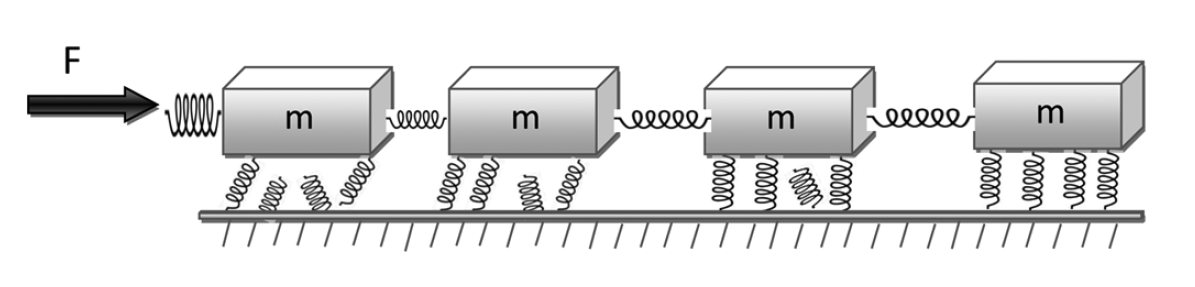
\includegraphics[width=0.5\linewidth]{figures/prl1.png}}



Grand challenge project in FYS-MEK1100 (Mechanics), Second Semester: a friction model to be solved as coupled ODEs. And find problems with the article?
\end{block}
\begin{block}{}


% inline figure
\centerline{
\includegraphics[width=0.5\linewidth]{figures/prl2.png}}


\end{block}
\end{frame}

\begin{frame}[plain,fragile]
\frametitle{Exciting possibilities}

\begin{block}{}

\textbf{At MSU with the new Department of Computational Mathematics, Science and Engineering we have a unique opportunity to include a computational perspective in our basic science education across disciplines, in addition to the educational programs that will be developed by the new department}.

\end{block}
\end{frame}

\begin{frame}[plain,fragile]
\frametitle{Modeling and computations as a way to enhance algorithminc thinking}

\begin{block}{}

Algorithmic  thinking as a way to

\begin{itemize}
\item Enhance instruction based teaching

\item Introduce Research based teaching  from day one

\item Trigger further insights in math and other disciplines 

\item Validation and verification of scientific results (the PRL example), with the possibility to emphasize ethical aspects as well. Version control is central.

\item Good working practices from day one.
\end{itemize}

\noindent
\end{block}
\end{frame}

\begin{frame}[plain,fragile]
\frametitle{Research based teaching}

\begin{block}{How do we define it? }
One possible definition: It is coupled to a direct participation in actual research and builds upon established
knowledge and insights about scientific methods.


\begin{itemize}
\item It is the standard situation at all universities  and takes normally place at the senior undergraduate/graduate level (isn't it too late?)

\item It is seldom done in undergraduate courses.

\item Taught by a researcher

\item The student starts seeing the countour of the scientific approach leading her/him to make new interpretations, develop new insights and understandings that lead  to further research.
\end{itemize}

\noindent
\end{block}
\end{frame}

\begin{frame}[plain,fragile]
\frametitle{Research based education}

\begin{block}{What should the education contain? }
The standard situation we meet at an almost daily basis:

\begin{itemize}
\item Theory+experiment+simulation is almost the norm in research and industry

\item To be able to model complex systems with no simple answers on closed form. Solve real problems.

\item Emphasis on insight and understanding of fundamental principles and laws in the Sciences.

\item Be able to visualize, present, discuss, interpret and come with a critical analysis of the results, and develop a sound ethical attitude to own and other's work.
\end{itemize}

\noindent
Our education should reflect this.
\end{block}
\end{frame}

\begin{frame}[plain,fragile]
\frametitle{Research based education}

\begin{block}{Normal workflow in Science and Engineering }

\begin{itemize}
\item A problem is properly described using a precise (normal) language.

\item It is translated to a mathematical problem using known laws and  principles.

\item It is solved, normally via numerical similations.

\item The solution is visualized and analyzed.

\item The solution to the problem is formulated.
\end{itemize}

\noindent
People who master these skills bring an important compentence to society. 
\end{block}
\end{frame}

\begin{frame}[plain,fragile]
\frametitle{Large scale simulations}

\begin{block}{Fluid dynamical simulations central in air industry.  Typical university courses which are taught address the physics of the lower left corner.  }


% inline figure
\centerline{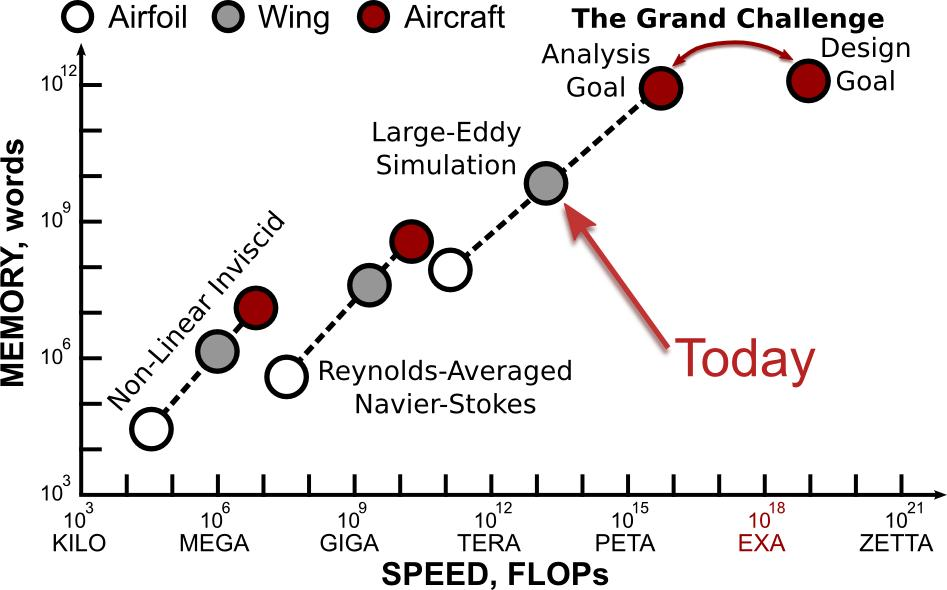
\includegraphics[width=0.6\linewidth]{figures/fig10.jpg}}


\end{block}
\end{frame}

\begin{frame}[plain,fragile]
\frametitle{Large scale simulations}

\begin{block}{}
Fluid dynamical simulations central in air industry, wings tested.


% inline figure
\centerline{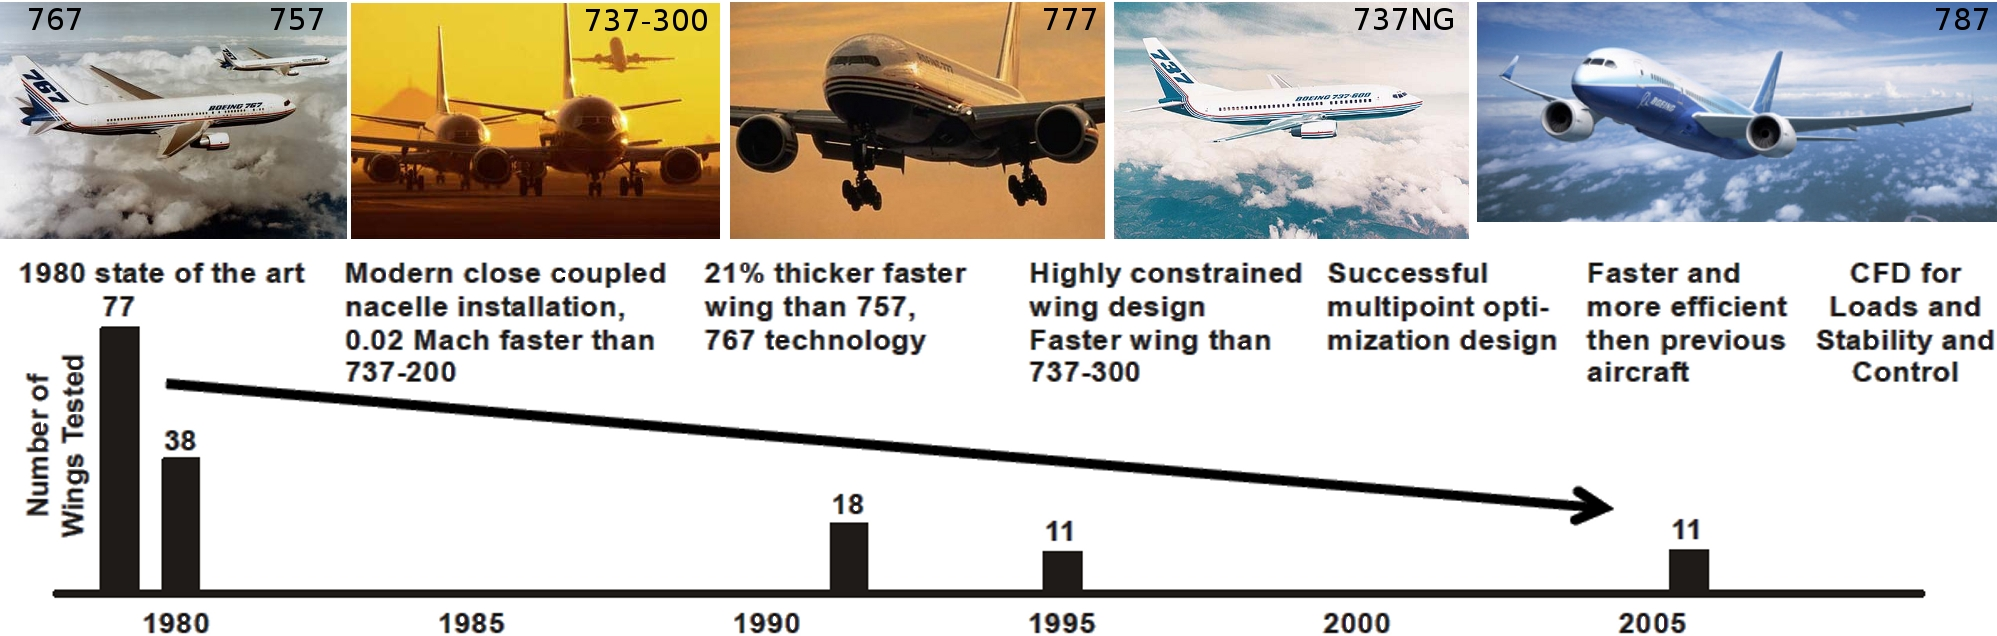
\includegraphics[width=1.0\linewidth]{figures/fig8.jpg}}


\end{block}
\end{frame}

\begin{frame}[plain,fragile]
\frametitle{Preliminary summary}

\begin{block}{Computations should enter basic science education }

\begin{itemize}
\item Computation is a fundamental tool to gain new insights and should be included in our elementary teaching.

\item Requires development of algorithmic thinking.

\item Basic numerical methods should be part of the compulsory curriculum.

\item The students should also learn to develop new numerical methods and adapt to new software tools.

\item Requires more training than simple programming in a mathematics course.
\end{itemize}

\noindent
\end{block}
\end{frame}

\begin{frame}[plain,fragile]
\frametitle{Can we catch many birds with one stone?}

\begin{block}{}
\begin{itemize}
\item How can we include and integrate an algorithmic (computational) perspective   in our basic education?

\item Can this enhance the students' understanding of mathematics and science?

\item Can it strengthen research based teaching?
\end{itemize}

\noindent
\end{block}
\end{frame}

\begin{frame}[plain,fragile]
\frametitle{What is needed?}

\begin{block}{Programming }
A compulsory programming course with a strong mathematical flavour. \emph{Should give a solid foundation in programming as a problem solving technique in mathematics}. Programming is understanding! The line of thought when solving mathematical problems numerically enhances algorithmic thinking,  and thereby the students' understanding of the scientific process.
\end{block}

\begin{block}{Mathematics and numerics }
Mathematics is at least as important as before, but should be supplemented with development, analysis, implementation, verification and validation of numerical methods. Science ethics and better understanding of the pedagogical process, almost for free!
\end{block}

\begin{block}{Sciences }
Training in modelling and problem solving with numerical methods and visualisation, as well as traditional methods in Science courses, Physics, Chemistry, Biology, Geology, Engineering...
\end{block}
\end{frame}

\begin{frame}[plain,fragile]
\frametitle{Implementation}

\begin{block}{Crucial ingredients }

\begin{itemize}
\item Support from governing bodies (now priority 1 of the College of Natural Science at UOslo)

\item Cooperation across departmental boundaries

\item Willingness by individuals to give priority to teaching reform
\end{itemize}

\noindent
Consensus driven approach.
\end{block}
\end{frame}

\begin{frame}[plain,fragile]
\frametitle{Implementation in Oslo: The CSE  project}

\begin{block}{What we do }
\begin{itemize}
\item Coordinated use of computational exercises and numerical tools in most undergraduate courses.

\item Help update the scientific staff's competence on computational aspects and give support (scientific, pedagogical and financial)  to those who wish to revise  their courses in a computational direction.

\item Teachers get good summer students to aid in introducing computational exercises

\item Develop courses and exercise modules with a computational perspective, both for students and teachers. 

\item Basic idea: mixture of mathematics, computation, informatics and topics from the physical sciences.
\end{itemize}

\noindent
Interesting outcome: higher focus on teaching and pedagogical issues!!
\end{block}
\end{frame}

\begin{frame}[plain,fragile]
\frametitle{Example of bachelor program, astrophysics}

\begin{block}{}


% inline figure
\centerline{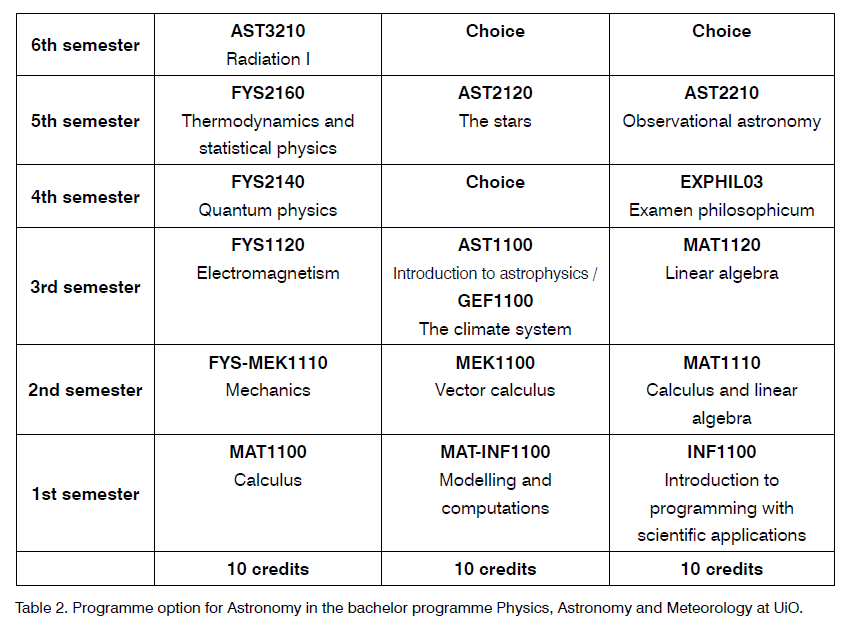
\includegraphics[width=0.6\linewidth]{figures/astronomy.png}}




\end{block}
\end{frame}

\begin{frame}[plain,fragile]
\frametitle{Example: Computations from day one}

\begin{block}{Differentiation }
Three courses the first semester:  MAT1100, MAT-INF1100 og INF1100.
\begin{itemize}
\item Definition  of the derivative in  MAT1100 (Calculus and analysis) 
\end{itemize}

\noindent
\[
 f'(x)=\lim_{h \rightarrow 0}\frac{f(x+h)-f(x)}{h}.
\]
\begin{itemize}
\item Algorithms to compute the derivative in MAT-INF1100  (Mathematical modelling with computing)
\end{itemize}

\noindent
\[
 f'(x)= \frac{f(x+h)-f(x-h)}{2h}+O(h^2).
\]
\begin{itemize}
\item Implementation in Python in INF1100
\end{itemize}

\noindent
\begin{minted}[fontsize=\fontsize{9pt}{9pt},linenos=false,mathescape,baselinestretch=1.0,fontfamily=tt,xleftmargin=2mm]{python}
def differentiate(f, x, h=1E-5):
     return (f(x+h) - f(x-h))/(2*h)
\end{minted}

\end{block}
\end{frame}

\begin{frame}[plain,fragile]
\frametitle{Example: Computations from day one}

\begin{block}{Differentiation and comparison with symbolic expressions }
Combined with the possibility of symbolic calculations with \emph{Sympy}, Python offers an environment where students and teachers alike can test many different aspects of mathematics and numerical mathematics, in addition to being able to verify and validate their codes. The following simple example shows how to extend the simple function for computing the numerical derivative with the possibility of obtaining the closed form or analytical expression
\begin{minted}[fontsize=\fontsize{9pt}{9pt},linenos=false,mathescape,baselinestretch=1.0,fontfamily=tt,xleftmargin=2mm]{python}
def differentiate(f, x, h=1E-5, symbolic=False):
    if symbolic:
        import sympy
        return sympy.lambdify([x], sympy.diff(f, x))
    else:
        return (f(x+h) - f(x-h))/(2*h)
\end{minted}

\end{block}
\end{frame}

\begin{frame}[plain,fragile]
\frametitle{Other Examples}

\begin{block}{Integration by Trapezoidal Rule  }

\begin{itemize}
\item Definition of integration  in MAT1100 (Calculus and analysis).

\item The algorithm for computing the  integral vha the Trapezoidal rule for an interval $x \in [a,b]$
\end{itemize}

\noindent
\[
  \int_a^b(f(x) dx \approx \frac{1}{2}\left [f(a)+2f(a+h)+\dots+2f(b-h)+f(b)\right] 
\]
\begin{itemize}
\item Taught   in MAT-INF1100  (Mathematical modelling)

\item The algorithm is then implemented in  INF1100 (programming course).
\end{itemize}

\noindent
\end{block}
\end{frame}

\begin{frame}[plain,fragile]
\frametitle{Typical implementation in INF1100}

\begin{block}{Integration by Trapezoidal Rule  }

\begin{minted}[fontsize=\fontsize{9pt}{9pt},linenos=false,mathescape,baselinestretch=1.0,fontfamily=tt,xleftmargin=2mm]{python}
from math import exp, log, sin
def Trapez(a,b,f,n):
   h = (b-a)/float(n)
   s = 0
   x = a
   for i in range(1,n,1):
       x = x+h
       s = s+ f(x)
   s = 0.5*(f(a)+f(b)) +s
   return h*s

def f1(x):
    return exp(-x*x)*log(1+x*sin(x))

a = 1;  b = 3; n = 1000
result = Trapez(a,b,f1,n)
print result
\end{minted}
\end{block}
\end{frame}

\begin{frame}[plain,fragile]
\frametitle{Typical implementation in INF1100}

\begin{block}{Symbolic calculations and numerical calculations in one code! }
Python offers an  extremely versatile programming  environment, allowing for the inclusion of analytical studies in a numerical program. Here we show another example
where \emph{SymPy} is used to evaluate the integral and compute the absolute error 
with respect to the numerically evaluated one of the integral
$4\int_0^1 dx/(1+x^2) = \pi$: 
\begin{minted}[fontsize=\fontsize{9pt}{9pt},linenos=false,mathescape,baselinestretch=1.0,fontfamily=tt,xleftmargin=2mm]{python}
from math import *
from sympy import *
def Trapez(a,b,f,n):
   h = (b-a)/float(n)
   s = 0
   x = a
   for i in range(1,n,1):
       x = x+h
       s = s+ f(x)
   s = 0.5*(f(a)+f(b)) +s
   return h*s

#  function to compute pi
def function(x):
    return 4.0/(1+x*x)

a = 0.0;  b = 1.0; n = 100
result = Trapez(a,b,function,n)
print "Trapezoidal rule=", result
# define x as a symbol to be used by sympy
x = Symbol('x')
exact = integrate(function(x), (x, 0.0, 1.0))
print "Sympy integration=", exact
# Find relative error
print "Relative error", abs((exact-result)/exact)
\end{minted}
\end{block}
\end{frame}

\begin{frame}[plain,fragile]
\frametitle{Integrating numerical mathematics with calculus}

\begin{block}{}
The last example shows the potential of combining numerical algorithms with symbolic calculations, allowing thereby students and teachers to

\begin{itemize}
\item Validate and verify  their  algorithms. 

\item Including concepts like unit testing, one has the possibility to test and validate several or all parts of the code.

\item Validation and verification are then included \emph{naturally} and one can develop a better attitude to what is meant with an ethically sound scientific approach.

\item The above example allows the student to also test the mathematical error of the algorithm for the trapezoidal rule by changing the number of integration points. The students get trained from day one to think error analysis. 

\item With an ipython notebook the students can keep exploring similar examples and turn them in as their own notebooks. 
\end{itemize}

\noindent
\end{block}
\end{frame}

\begin{frame}[plain,fragile]
\frametitle{Error analysis}

\begin{block}{}
The following extended version of the trapezoidal rule allows the student to plot the relative error by comparing with the exact result. By increasing to $10^8$ points one arrives at a region where numerical errors start to accumulate.
\begin{minted}[fontsize=\fontsize{9pt}{9pt},linenos=false,mathescape,baselinestretch=1.0,fontfamily=tt,xleftmargin=2mm]{python}
from math import log10
import numpy as np
from sympy import Symbol, integrate
import matplotlib.pyplot as plt
# function for the trapezoidal rule
def Trapez(a,b,f,n):
   h = (b-a)/float(n)
   s = 0
   x = a
   for i in range(1,n,1):
       x = x+h
       s = s+ f(x)
   s = 0.5*(f(a)+f(b)) +s
   return h*s
#  function to compute pi
def function(x):
    return 4.0/(1+x*x)
# define integration limits
a = 0.0;  b = 1.0;
# find result from sympy
# define x as a symbol to be used by sympy
x = Symbol('x')
exact = integrate(function(x), (x, a, b))
# set up the arrays for plotting the relative error
n = np.zeros(8); y = np.zeros(8);
# find the relative error as function of integration points
for i in range(0, 8, 1):
    npts = 10**i
    result = Trapez(a,b,function,npts)
    RelativeError = abs((exact-result)/exact)
    n[i] = log10(npts); y[i] = log10(RelativeError);   
plt.plot(n,y, 'ro')
plt.xlabel('n')
plt.ylabel('Relative error')
plt.show()
\end{minted}
\end{block}
\end{frame}

\begin{frame}[plain,fragile]
\frametitle{Additional benefits: A structured approach to solving problems}

\begin{block}{}
In this process we easily bake in
\begin{enumerate}
  \item How to structure a code in terms of functions

  \item How to make a module

  \item How to read input data flexibly from the command line

  \item How to create graphical/web user interfaces

  \item How to write unit tests (test functions or doctests)

  \item How to refactor code in terms of classes (instead of functions only)

  \item How to conduct and automate large-scale numerical experiments

  \item How to write scientific reports in various formats ({\LaTeX}, HTML)
\end{enumerate}

\noindent
\end{block}
\end{frame}

\begin{frame}[plain,fragile]
\frametitle{Additional benefits: A structure approach to solving problems}

\begin{block}{}
The conventions and techniques outlined here will save you a lot of time when you incrementally extend software over time from simpler to more complicated problems. In particular, you will benefit from many good habits:
\begin{enumerate}
\item New code is added in a modular fashion to a library (modules)

\item Programs are run through convenient user interfaces

\item It takes one quick command to let all your code undergo heavy testing 

\item Tedious manual work with running programs is automated,

\item Your scientific investigations are reproducible, scientific reports with top quality typesetting are produced both for paper and electronic devices.
\end{enumerate}

\noindent
\end{block}
\end{frame}

\begin{frame}[plain,fragile]
\frametitle{Learning outcomes three first semesters}

\begin{block}{Knowledge of basic algorithms }

\begin{itemize}
\item Differential equations: Euler, modified Euler and Runge-Kutta methods (first semester)

\item Numerical integration: Trapezoidal and Simpson's rule, multidimensional integrals (first semester)

\item Random numbers, random walks, probability distributions and Monte Carlo integration  (first semester)

\item Linear Algebra and eigenvalue problems: Gaussian elimination, LU-decomposition, SVD, QR, Givens rotations and eigenvalues, Gauss-Seidel. (second and third semester)

\item Root finding and interpolation etc. (all three first semesters)

\item Processing of sound and images (first semester).
\end{itemize}

\noindent
The students have to code several of these algorithms during the first three semesters.
\end{block}
\end{frame}

\begin{frame}[plain,fragile]
\frametitle{Later courses}

\begin{block}{}

\textbf{Later courses should build on this foundation as much as possible}.

\begin{enumerate}
\item In particular, the course should not be too basic! There should be progression in the use of mathematics, numerical methods and programming, as well as science.

\item Computational platform: Python, fully object-oriented and allows for seamless integration of c++ and Fortran codes, as well as Matlab-like programming environment. Makes it easy to parallelize codes as well.
\end{enumerate}

\noindent
\end{block}
\end{frame}

\begin{frame}[plain,fragile]
\frametitle{Coordination}

\begin{block}{}
\begin{itemize}
\item Teachers in other courses need therefore not use much time on numerical tools. Naturally included in other courses.
\end{itemize}

\noindent
\end{block}
\end{frame}

\begin{frame}[plain,fragile]
\frametitle{FYS-MEK1100 (Mechanics), Second Semester}

\begin{block}{Realistic Pendulum }

Classical pendulum with damping and external force
\[
  ml\frac{d^2\theta}{dt^2}+\nu\frac{d\theta}{dt}  +mgsin(\theta)=Asin(\omega t).
\]
Easy to solve numerically without classical simplification, and then visualize the solution.  Done in first semester!
Same equation for an RLC circuit 
\[
L\frac{d^2Q}{dt^2}+\frac{Q}{C}+R\frac{dQ}{dt}=V(t).
\]
\end{block}
\end{frame}

\begin{frame}[plain,fragile]
\frametitle{FYS1120 Electromagnetism, Third Semester}

\begin{block}{RLC circuit }
Same equation as the pendulum for an RLC circuit 
\[
L\frac{d^2Q}{dt^2}+\frac{Q}{C}+R\frac{dQ}{dt}=V(t).
\]
From the numerics, 
the students found the optimal parameters for studying experimentally chaos
in an RLC circuit. Then they did the experiment.

\end{block}
\end{frame}

\begin{frame}[plain,fragile]
\frametitle{More Examples from Physics Courses, 2-5 semester}

\begin{block}{Second-fourth semester }

\begin{itemize}
\item Air resistance in two and three dimensions with quadratic velocity dependence.

\item Launching a probe into a tornado

\item Rocket launching with realistic parameters, gravity assist

\item How to kick a football and model its trajectory.

\item Planet motion and position of planets

\item Magnetic fields with various geometries based on Biot-Savart's law

\item Harmonic oscillations and various forms of electromagnetic waves.

\item Combined effect of different potentials such as the electrostatic potential and the gravitational potential.

\item Simple studies of atoms and molecules, and much more
\end{itemize}

\noindent
\end{block}
\end{frame}

\begin{frame}[plain,fragile]
\frametitle{First computational physics course}

\begin{block}{Late: Fifth semester, FYS3150 Computational Physics }

The first computational physics \href{{http://www.uio.no/studier/emner/matnat/fys/FYS3150/h14/}}{course} can then be used to summarize many of the gained insights about algorithms, mathematical models, physics etc. And direct the students to more advanced algorithms and applications like

\begin{itemize}
\item Monte carlo methods

\item Parallelization

\item Solving quantum mechanical problems by Variational Monte Carlo  or other quantum mechanical methods

\item Study phase transitions with for example the Ising and Potts model.

\item Molecular dynamics simulations etc etc 
\end{itemize}

\noindent
\end{block}
\end{frame}

\begin{frame}[plain,fragile]
\frametitle{Challenges...}

\begin{block}{.. and objections }

\emph{Standard objection: computations take away the attention from other central topics in 'my course'}. 

CSE incorporates computations from day one, and courses higher up do not need to
spend time on computational topics  (technicalities), but can focus on the interesting
science applications.

\begin{itemize}
\item To help teachers: Developed pedagogical modules which can aid university teachers.
\end{itemize}

\noindent
\end{block}
\end{frame}

\begin{frame}[plain,fragile]
\frametitle{Challenges and future plans}

\begin{block}{}

\begin{itemize}
\item The project depends crucially on few individuals. 

\item Need to get more teachers involved, not only good TAs.

\item How  to implement a CSE perspective in other programs like Chemistry, Molecular Biology,  Biology, Engineering. New courses are being developed.

\item Now a national pilot for other universities and regional colleges.
\end{itemize}

\noindent
\textbf{Key issue: modularization of topics and development of a 'technological platform' which glues together different modules}

\end{block}
\end{frame}

\begin{frame}[plain,fragile]
\frametitle{Which aspects are important for a successful introduction of CSE?}

\begin{block}{}

\begin{itemize}
\item Early introduction, programming course at beginning of studies linked with math courses and science and engineering courses.

\item Crucial to learn proper programming at the beginning.

\item Good TAs

\item Choice of software.

\item Textbooks and modularization of topics.

\item Resources and expenses.

\item Tailor to specific disciplines.

\item Organizational matters.
\end{itemize}

\noindent
\end{block}
\end{frame}

\begin{frame}[plain,fragile]
\frametitle{What about life science/biology? Overarching questions}

\pause
\begin{block}{Which skills are needed by candidates in biology? }
There is new demand for more

\begin{itemize}
  \item quantitative methods {\&} reasoning

  \item understanding data and phenomena via models

  \item creating \emph{in silico} virtual labs
\end{itemize}

\noindent
\end{block}

\pause
\begin{block}{Challenge: }
How to integrate such computing-based activities in the undergraduate programs
when the students are \emph{not} interested in mathematics, physics, and
programming?
\end{block}
\end{frame}

\begin{frame}[plain,fragile]
\frametitle{How to teach computing in biology?}

\pause
\begin{block}{}
Do we need to still follow the tradition and teach mathematics, physics, computations, chemistry, etc. in separate discipline-specific courses?

\begin{itemize}
  \item Uninteresting to first study tools when you want to study biology

  \item Little understanding of what the tools are good for

  \item Minor utilization of tools later in biology
\end{itemize}

\noindent
\end{block}

\pause
\begin{block}{It's time for new thinking: }
\begin{itemize}
  \item Just-in-time teaching: teach tools \emph{when needed}

  \item Teach tools in the \emph{context of biology}

  \item Emphasize development of \emph{intuition and understanding}

  \item Base learning of the students' own \emph{explorations in biology projects}

  \item Integrate lab work with computing tools
\end{itemize}

\noindent
\end{block}
\end{frame}

\begin{frame}[plain,fragile]
\frametitle{The pedagogical framework}

\begin{block}{Aim: Develop intuition about the scientific method }
\begin{itemize}
 \item Method: case-based learning

 \item Coherent problem solving \emph{in biology} by integrating
   mathematics, programming, physics/chemistry, ...

 \item Starting point: data from lab or field experiments

 \item Visualize data

 \item Derive computational models directly from mathematical/intuitive \emph{reasoning}

 \item Program model(s), fit parameters, compare with data

 \item Develop intuition and understanding based on
\begin{itemize}

  \item the principles behind the model

  \item exploration of the model (``what if'')

  \item prediction of new experiments
\end{itemize}

\noindent
\end{itemize}

\noindent
\end{block}
\end{frame}

\begin{frame}[plain,fragile]
\frametitle{Example 1: ecoli lab experiment}

\begin{block}{}
Observations of no of bacteria vs time in seconds,
stored in Excel and written to a CVS file:

\begin{minted}[fontsize=\fontsize{9pt}{9pt},linenos=false,mathescape,baselinestretch=1.0,fontfamily=tt,xleftmargin=2mm]{text}
0,100
600,140
1200,250
1800,360
2400,480
3000,820
3600,1300
4200,1700
4800,2900
5400,3900
6000,7000
\end{minted}
\end{block}
\end{frame}

\begin{frame}[plain,fragile]
\frametitle{Visualize data}

\begin{block}{}
\begin{itemize}
 \item Meet a text editor and a terminal window

 \item Very basic Unix
\end{itemize}

\noindent
First program:

\begin{minted}[fontsize=\fontsize{9pt}{9pt},linenos=false,mathescape,baselinestretch=1.0,fontfamily=tt,xleftmargin=2mm]{python}
t = [0, 600, 1200, 1800, 2400, 3000, 3600,
     4200, 4800, 5400, 6000]
N = [100, 140, 250, 360, 480, 820, 1300, 1700, 2900, 3900, 7000]
import matplotlib.pyplot as plt
plt.plot(t, N, 'ro')
plt.xlabel('t [s]')
plt.ylabel('N')
plt.show()
\end{minted}
\end{block}
\end{frame}

\begin{frame}[plain,fragile]
\frametitle{Concepts must be introduced implicitly in a structured way}

\begin{block}{Warning}
\begin{itemize}
 \item Always identify new concepts

 \item Train new concepts in simplified (``trivial'') problems
\end{itemize}

\noindent
\end{block}

\begin{block}{Concepts in the previous example: }
\begin{itemize}
 \item Lists or arrays of numbers

 \item Plotting commands

 \item Curve = function of time
\end{itemize}

\noindent
\end{block}

\begin{block}{Notice: }
The concept of a continuous function $N(t)$ is not necessary,
just straight lines between discrete points on a curve.
\end{block}
\end{frame}

\begin{frame}[plain,fragile]
\frametitle{Read data from file}

\begin{block}{}
\begin{minted}[fontsize=\fontsize{9pt}{9pt},linenos=false,mathescape,baselinestretch=1.0,fontfamily=tt,xleftmargin=2mm]{python}
import numpy as np
data = np.loadtxt('ecoli.csv', delimiter=',')
print data  # look at the format
t = data[:,0]
N = data[:,1]
import matplotlib.pyplot as plt
plt.plot(t, N, 'ro')
plt.xlabel('t [s]')
plt.ylabel('N')
plt.show()
\end{minted}
\end{block}

\begin{block}{Typical pattern: }
The population grows faster and faster. Why? Is there an
underlying (general) mechanism?
\end{block}
\end{frame}

\begin{frame}[plain,fragile]
\frametitle{Lab journal}

\begin{block}{}
Use IPython notebook as lab journal.
\end{block}
\end{frame}

\begin{frame}[plain,fragile]
\frametitle{How can we reason about the process?}

% \href{{http://www.zo.utexas.edu/courses/Thoc/PopGrowth.html}}{\nolinkurl{http://www.zo.utexas.edu/courses/Thoc/PopGrowth.html}}

\begin{block}{}
\begin{enumerate}
\pause
\item Cells divide after $T$ seconds on average (one generation)

\pause
\item $2N$ celles divide into twice as many new cells $\Delta N$ in a time
   interval $\Delta t$ as $N$ cells would: $\Delta N \propto N$

\pause
\item $N$ cells result in twice as many new individuals $\Delta N$ in
   time $2\Delta t$ as in time $\Delta t$: $\Delta N \propto\Delta t$

\pause
\item Same proportionality wrt death (repeat reasoning)

\pause
\item Proposed model: $\Delta N = b\Delta t N - d\Delta tN$ for some unknown
   constants $b$ (births) and $d$ (deaths)

\pause
\item Describe evolution in discrete time: $t_n=n\Delta t$

\pause
\item Program-friendly notation: $N$ at $t_n$ is $N^n$

\pause
\item Math model: $N^{n+1} = N^n + r\Delta t\, N$ (with $\ r=b-d$)

\pause
\item Program model: \Verb!N[n+1] = N[n] + r*dt*N[n]!
\end{enumerate}

\noindent
\end{block}
\end{frame}

\begin{frame}[plain,fragile]
\frametitle{The first simple program}

\begin{block}{}
Let us solve the difference equation in as simple way as possible,
just to train some programming: $r=1.5$, $N^0=1$, $\Delta t=0.5$

\begin{minted}[fontsize=\fontsize{9pt}{9pt},linenos=false,mathescape,baselinestretch=1.0,fontfamily=tt,xleftmargin=2mm]{python}
import numpy as np

t = np.linspace(0, 10, 21)  # 20 intervals in [0, 10]
dt = t[1] - t[0]
N = np.zeros(t.size)

N[0] = 1
r = 0.5

for n in range(0, N.size-1, 1):
    N[n+1] = N[n] + r*dt*N[n]
    print 'N[%d]=%.1f' % (n+1, N[n+1])
\end{minted}
\end{block}
\end{frame}

\begin{frame}[plain,fragile]
\frametitle{The output}

\begin{Verbatim}[numbers=none,fontsize=\fontsize{9pt}{9pt},baselinestretch=0.95]
N[1]=1.2
N[2]=1.6
N[3]=2.0
N[4]=2.4
N[5]=3.1
N[6]=3.8
N[7]=4.8
N[8]=6.0
N[9]=7.5
N[10]=9.3
N[11]=11.6
N[12]=14.6
N[13]=18.2
N[14]=22.7
N[15]=28.4
N[16]=35.5
N[17]=44.4
N[18]=55.5
N[19]=69.4
N[20]=86.7
\end{Verbatim}
\end{frame}

\begin{frame}[plain,fragile]
\frametitle{Parameter estimation}

\begin{block}{}
\begin{itemize}
 \item We do not know $r$

 \item How can we estimate $r$ from data?
\end{itemize}

\noindent
We can use the difference equation with the experimental data

\[ N^{n+1} = N^n + r\Delta t N^n\]
Say $N^{n+1}$ and $N^n$ are known from data, solve wrt $r$:

\[ r = \frac{N^{n+1}-N^n}{N^n\Delta t} \]

Use experimental data in the fraction, say $t_1=600$, $t_2=1200$,
$N^1=140$, $N^2=250$: $r=0.0013$.
\end{block}

\begin{block}{More sophisticated methods }
Can do a nonlinear least squares parameter fit, but that is
too advanced at this stage.
\end{block}
\end{frame}

\begin{frame}[plain,fragile]
\frametitle{A program relevant for the biological problem}

% exact r = 0.000694

\begin{block}{}
\begin{minted}[fontsize=\fontsize{9pt}{9pt},linenos=false,mathescape,baselinestretch=1.0,fontfamily=tt,xleftmargin=2mm]{python}
import numpy as np

# Estimate r
data = np.loadtxt('ecoli.csv', delimiter=',')
t_e = data[:,0]
N_e = data[:,1]
i = 2  # Data point (i,i+1) used to estimate r
r = (N_e[i+1] - N_e[i])/(N_e[i]*(t_e[i+1] - t_e[i]))
print 'Estimated r=%.5f' % r
# Can experiment with r values and see if the model can
# match the data better

T = 1200     # cell can divide after T sec
t_max = 5*T  # 5 generations in experiment
t = np.linspace(0, t_max, 1000)
dt = t[1] - t[0]
N = np.zeros(t.size)

N[0] = 100
for n in range(0, len(t)-1, 1):
    N[n+1] = N[n] + r*dt*N[n]

import matplotlib.pyplot as plt
plt.plot(t, N, 'r-', t_e, N_e, 'bo')
plt.xlabel('time [s]');  plt.ylabel('N')
plt.legend(['model', 'experiment'], loc='upper left')
plt.show()
\end{minted}

Change \Verb!r! in the program and play around to make a better fit!
\end{block}
\end{frame}

\begin{frame}[plain,fragile]
\frametitle{Discuss the nature of such a model}

\begin{block}{}
\begin{itemize}
 \item Write up all the biological factors that influence the
   population size of bacteria

 \item Understand that all such effects are merged into one parameter $r$

 \item Understand that the reasoning must be the same whether we
   have bacteria, animals or humans - this is a generic model!\\
   (even the interest rate in a bank follows the same model)
\end{itemize}

\noindent
\end{block}
\end{frame}

\begin{frame}[plain,fragile]
\frametitle{Discuss the limitations of such a model}

\begin{block}{}
\begin{itemize}
 \item How many bacteria in the lab after one month?

 \item Growth is restricted by environmental resources!

 \item Fix the model (logistic growth)

 \item Is the logistic model appropriate for a lab experiment?

 \item Find data to support the logistic model \\
   (it's a \emph{very} simple model)
\end{itemize}

\noindent
\end{block}
\end{frame}

\begin{frame}[plain,fragile]
\frametitle{The pedagogical template (to be iterated!)}

\begin{block}{}
\begin{itemize}
 \item Start with a real biological problem

 \item Be careful with too many new concepts

 \item Workflow:
\begin{itemize}

  \item data

  \item visualization

  \item patterns

  \item modeling (\emph{discrete})

  \item programming

  \item testing

  \item parameter estimation (difficult)

  \item validation

  \item prediction

\end{itemize}

\noindent
 \item Make many small exercises that train the new concepts

 \item Repeat the case in a way that makes a complete understanding
\end{itemize}

\noindent
\end{block}
\end{frame}

\begin{frame}[plain,fragile]
\frametitle{Do we get better students?}

\begin{block}{Molecular dynamics visualization by two MSc students }


% inline figure
\centerline{\includegraphics[width=0.7\linewidth]{figures/visualize.jpg}}



% \includegraphics[width=9.5cm]{visualize.jpg}

\end{block}
\end{frame}

\begin{frame}[plain,fragile]
\frametitle{Summary}

\begin{block}{}

\begin{itemize}
\item Make our research visible in early undergraduate courses, enhance research based teaching

\item Possibility to focus more on understanding and increased insight.

\item Impetus for broad cooperation in teaching.

\item Strengthening of instruction based teaching (expensive and time-consuming).

\item Give our candidates a broader and more up-to-date education with a problem-based orientation, often requested by potential employers.

\item And perhaps the most important issue: does this enhance the student's insight in the Sciences?
\end{itemize}

\noindent
\end{block}
\end{frame}

\begin{frame}[plain,fragile]
\frametitle{People and links}

\begin{block}{}
\begin{itemize}
\item Hans Petter Langtangen, Computer Science

\item Knut Morken, Mathematics

\item Anders Malthe Sorensen and Arnt Inge Vistnes, Physics

\item Tom Lindstrom, Mathematics

\item Oyvind Ryan, Mathematics

\item Solveig Kristensen, Dean of Education

\item Hanne Solna, Director of studies

\item \href{{http://www.mn.uio.no/english/about/collaboration/cse/}}{\nolinkurl{http://www.mn.uio.no/english/about/collaboration/cse/}}

\item \href{{http://www.mn.uio.no/english/about/collaboration/cse/national-group/computing-in-science-education.pdf}}{\nolinkurl{http://www.mn.uio.no/english/about/collaboration/cse/national-group/computing-in-science-education.pdf}}
\end{itemize}

\noindent
\end{block}
\end{frame}

\begin{frame}[plain,fragile]
\frametitle{More links}

\begin{block}{}
\begin{itemize}
\item Python and our first programming course, first semester \href{{http://www.uio.no/studier/emner/matnat/ifi/INF1100/h14/}}{course}. Excellent new textbook by Hans Petter Langtangen, click here for the \href{{http://www.amazon.com/Scientific-Programming-Computational-Science-Engineering-ebook/dp/B00DGER1NQ/ref=sr_1_2?ie=UTF8&qid=1425382942&sr=8-2&keywords=langtangen}}{textbook} or the \href{{http://hplgit.github.io/primer.html/doc/web/index.html}}{online version}

\item Mathematical modelling course, first semester \href{{http://www.uio.no/studier/emner/matnat/math/MAT-INF1100/h14/}}{course}. Textbook by Knut Morken to be published by Springer.

\item Mechanics, second semester \href{{http://www.uio.no/studier/emner/matnat/fys/FYS-MEK1100/v12/}}{course}. New textbook by Anders Malthe-Sorenssen, in press by Springer, Undergraduate Lecture Notes in Physics

\item Computational Physics I, fifth semester \href{{http://www.uio.no/studier/emner/matnat/fys/FYS3150/h14/}}{course}. Textbook to be published by IOP in 2015, with \href{{http://www.uio.no/studier/emner/matnat/fys/FYS3150/h14/undervisningsmateriale/Lecture%20Notes/lecture2014.pdf}}{online version}.
\end{itemize}

\noindent
\end{block}
\end{frame}

\end{document}
